\documentclass[]{report}
\usepackage{amsmath}
\usepackage{graphicx}
\usepackage{tabularx}
\usepackage{amsfonts}
\usepackage{amssymb}
\usepackage{amsbsy}

% Title Page
\title{MachineLearning for Visual Computing Aufgabenblock 1}
\author{Christian Br\"andle}


\begin{document}
\maketitle

\begin{abstract}
\end{abstract}

\section{Einfaches Perceptron - Datengeneration}

%My_1 = [10, 10,10,10]; 
%Sigma_1 = [5,4,3,2];
%My_2 = [2, 2, 2, 2]; 
%Sigma_2 = [2,3,4,5];

Gegeben sind vier Datensets a 100 Beobachtungen von 2-dimensionalen Eingangsdaten, welche normalverteilt sind. Die Entscheidungsgrenze 

\begin{figure}[p]
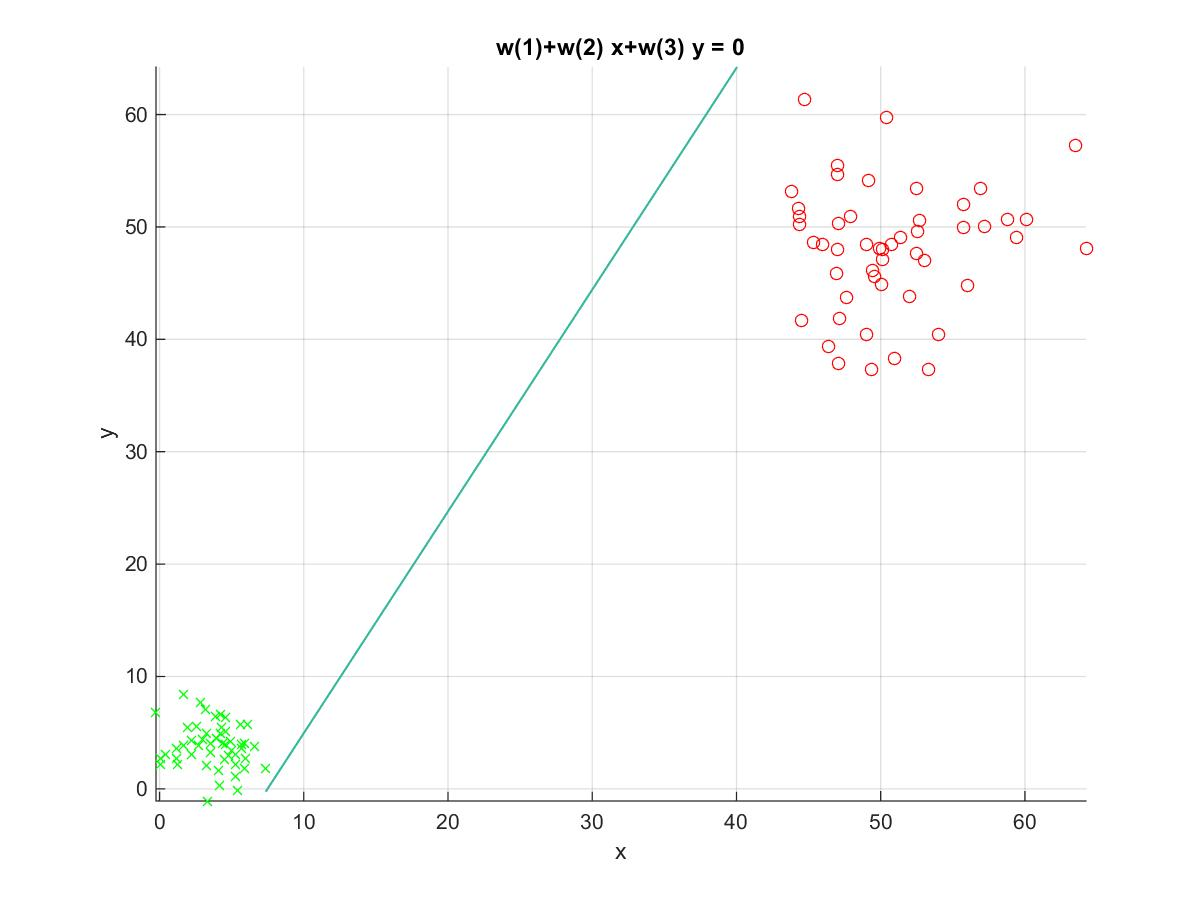
\includegraphics[width=0.7\textwidth]{./images/MyPerceptron_1.jpg}
\caption{Datensatz 1: $\mu_1=10$, $\Sigma_1=5$ , Datensatz 2: $\mu_2=2$, $\Sigma_2=2$}
\end{figure}

\begin{figure}[p]
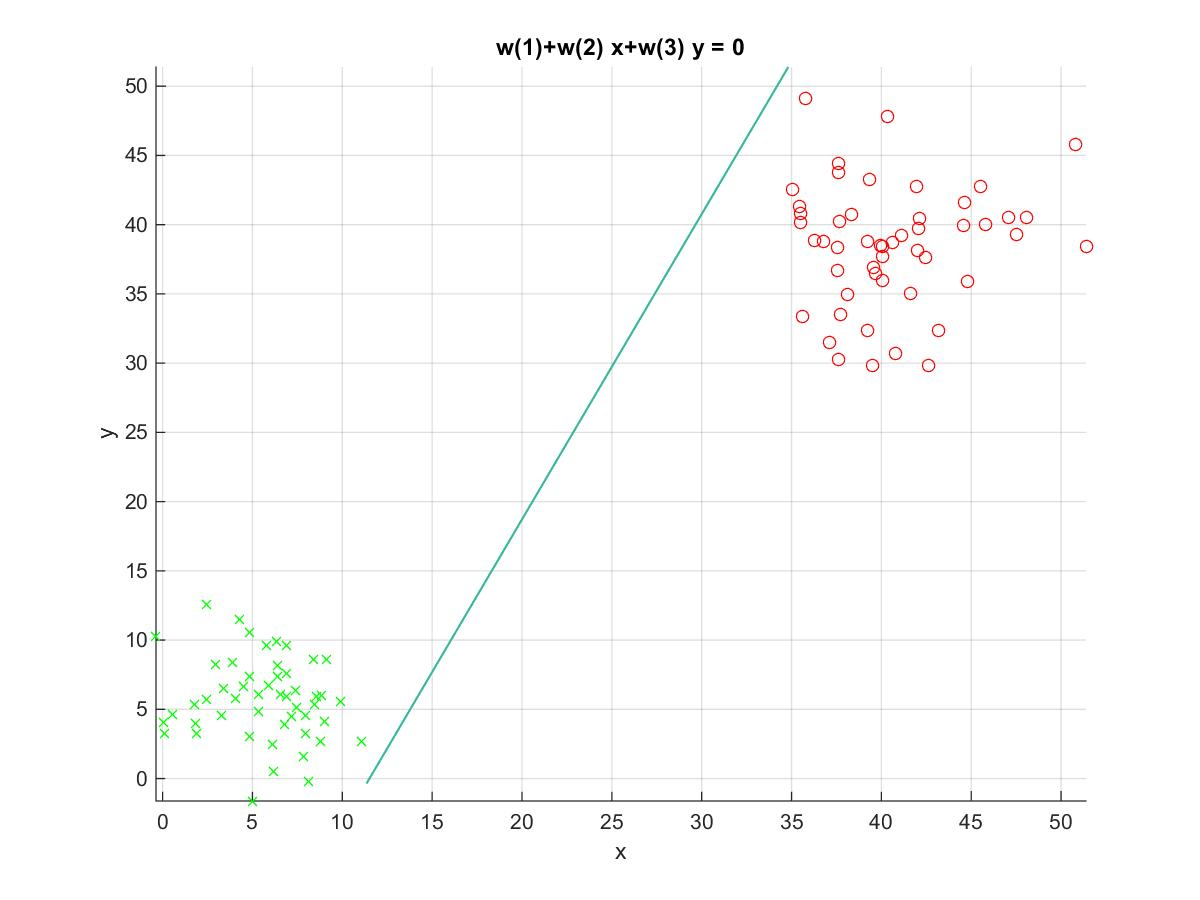
\includegraphics[width=0.7\textwidth]{./images/MyPerceptron_2.jpg}
\caption{Datensatz 1: $\mu_1=10$, $\Sigma_1=4$ , Datensatz 2: $\mu_2=2$, $\Sigma_2=3$}
\end{figure}

\begin{figure}[p]
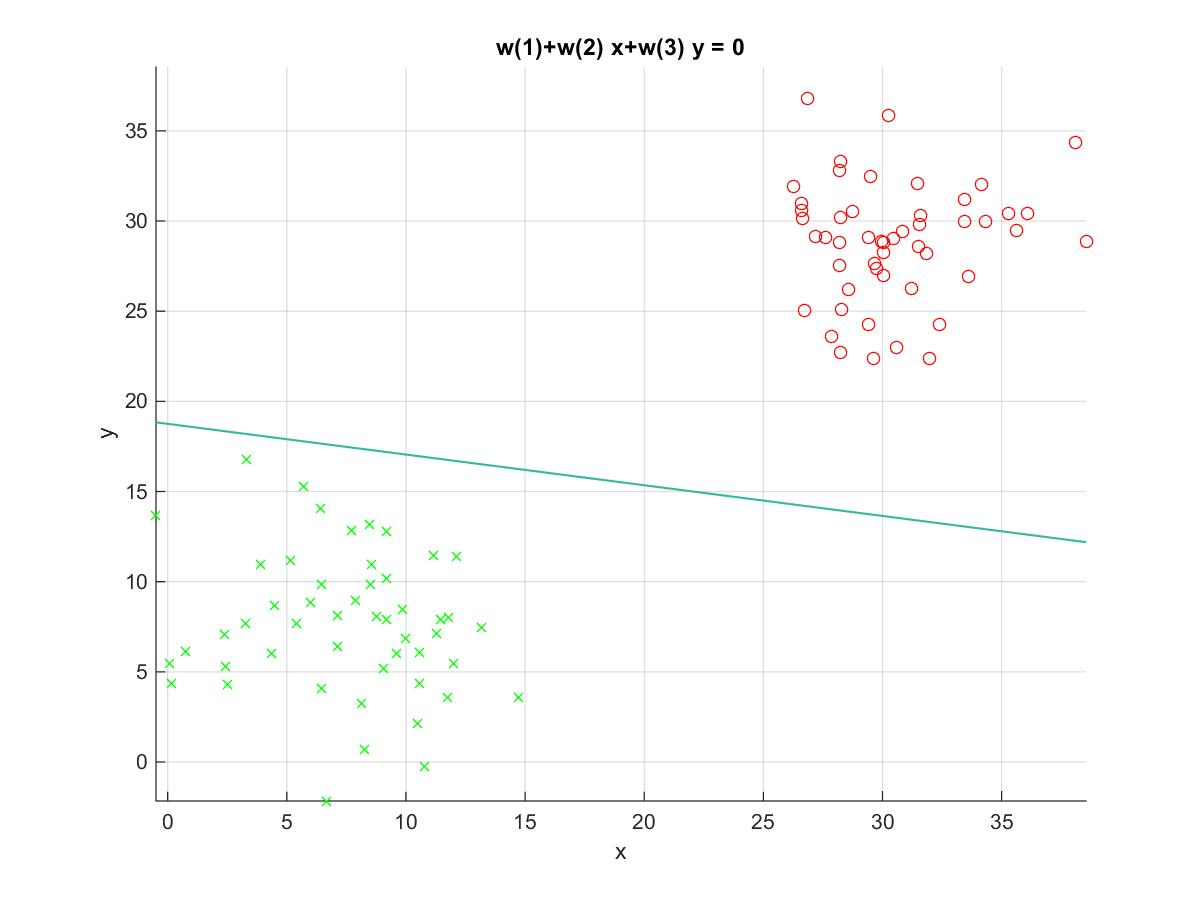
\includegraphics[width=0.7\textwidth]{./images/MyPerceptron_3.jpg}
\caption{Datensatz 1: $\mu_1=10$, $\Sigma_1=3$ , Datensatz 2: $\mu_2=2$, $\Sigma_2=4$}
\end{figure}

\begin{figure}[p]
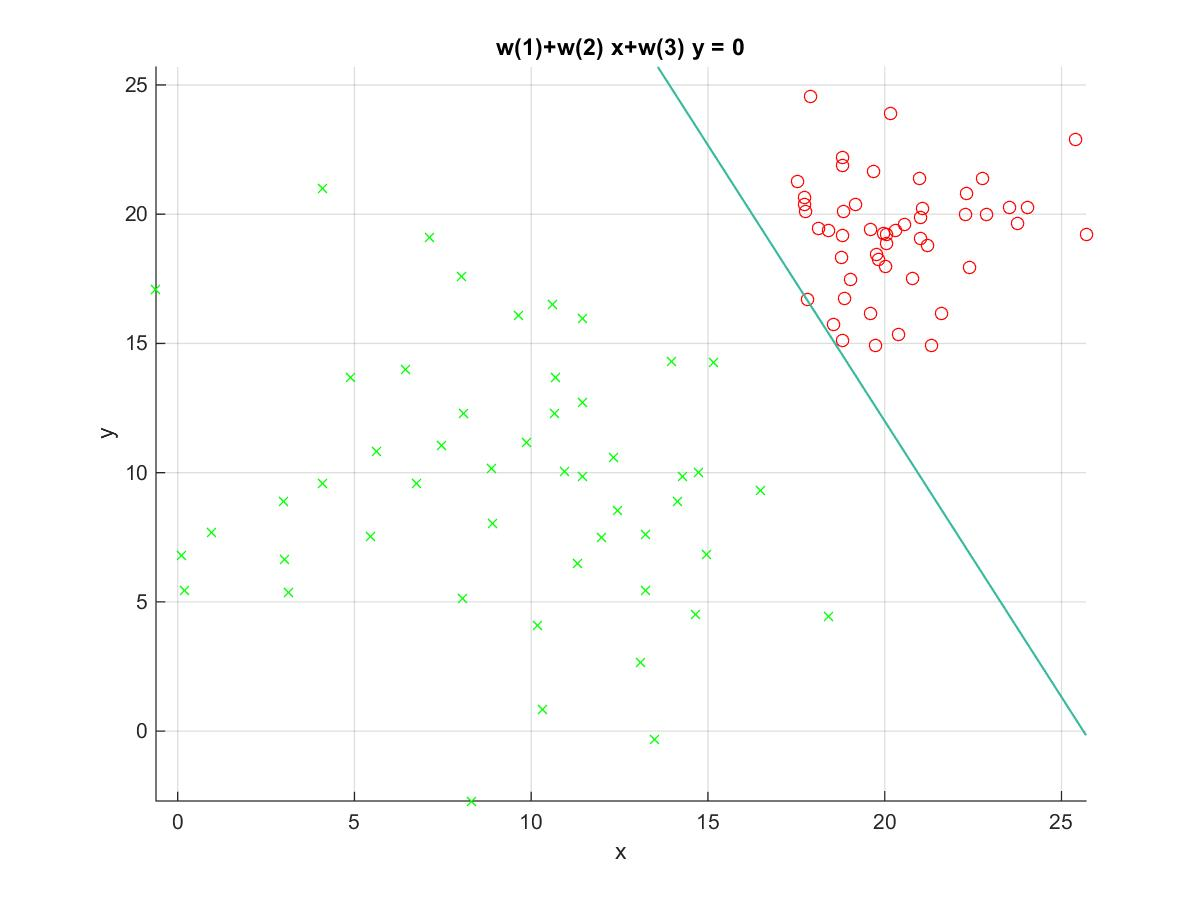
\includegraphics[width=0.7\textwidth]{./images/MyPerceptron_4.jpg}
\caption{Datensatz 1: $\mu_1=10$, $\Sigma_1=2$ , Datensatz 2: $\mu_2=2$, $\Sigma_2=5$}
\end{figure}

%\begin{tabular}{| l | l |}
%\hline
%\hline
%\end{tabular}

\section{Einfaches Perceptron - Perceptrontraining}

\subsection{Daten und Entscheidungsgrenzen im $\mathbb{R}^2$}

\begin{figure}[p]
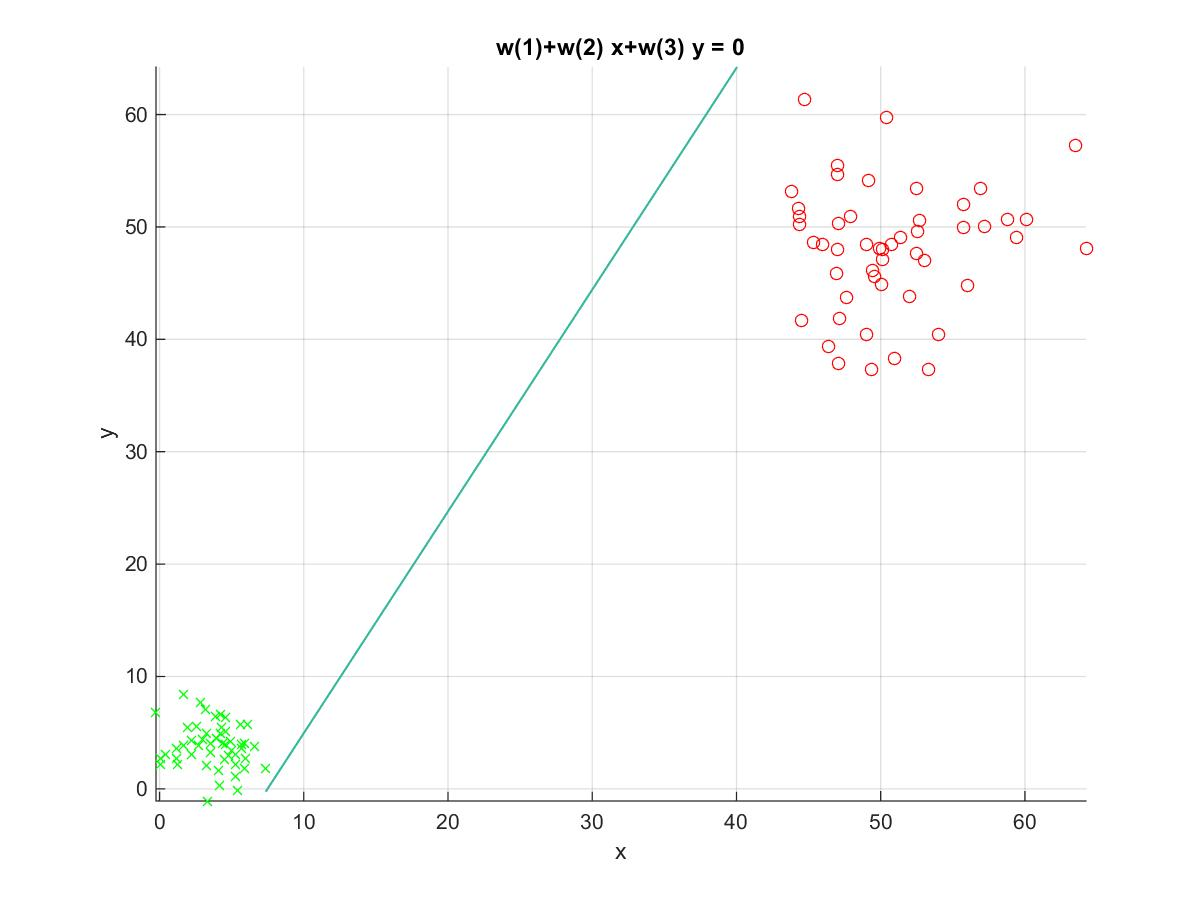
\includegraphics[width=0.7\textwidth]{./images/MyPerceptron_1.jpg}
\caption{Datensatz 1: $\mu_1=10$, $\Sigma_1=5$ , Datensatz 2: $\mu_2=2$, $\Sigma_2=2$}
\end{figure}

\begin{figure}[p]
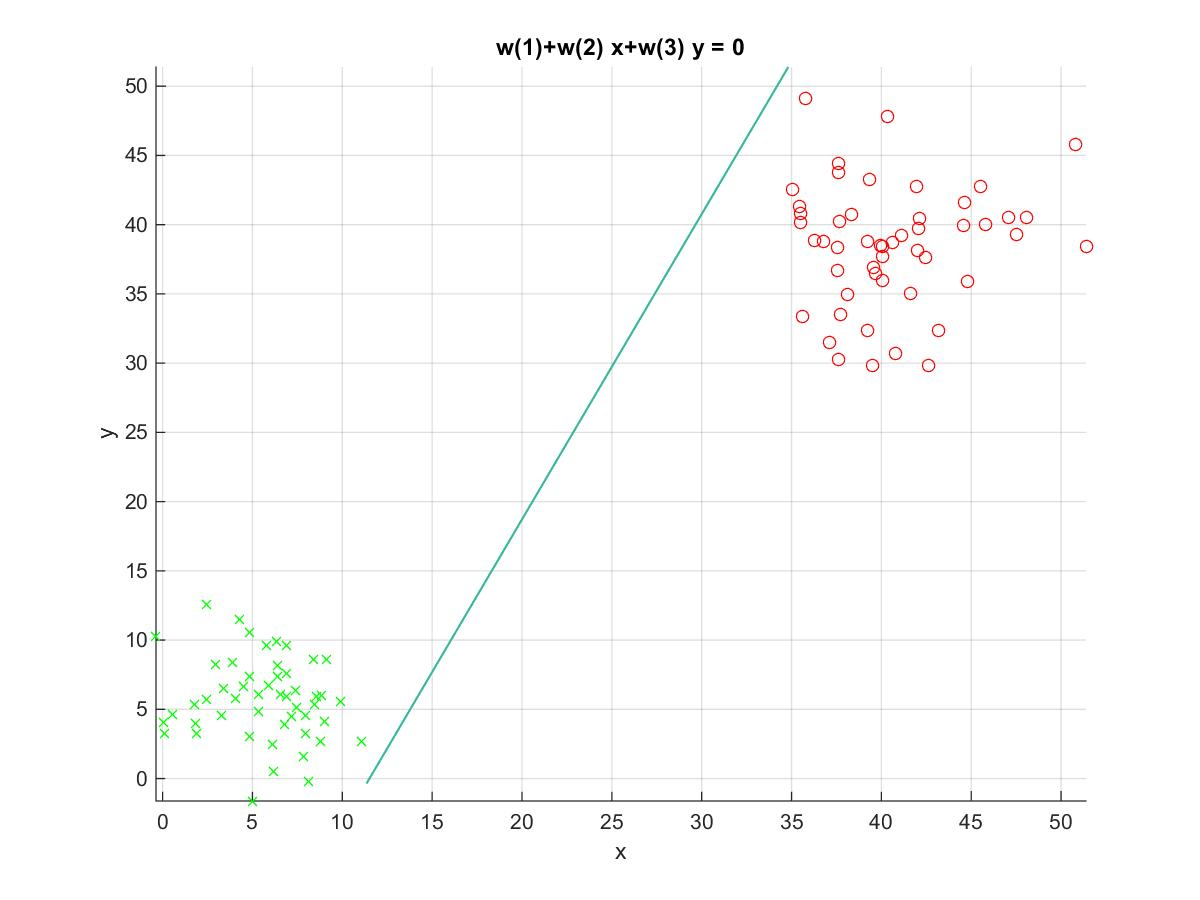
\includegraphics[width=0.7\textwidth]{./images/MyPerceptron_2.jpg}
\caption{Datensatz 1: $\mu_1=10$, $\Sigma_1=4$ , Datensatz 2: $\mu_2=2$, $\Sigma_2=3$}
\end{figure}

\begin{figure}[p]
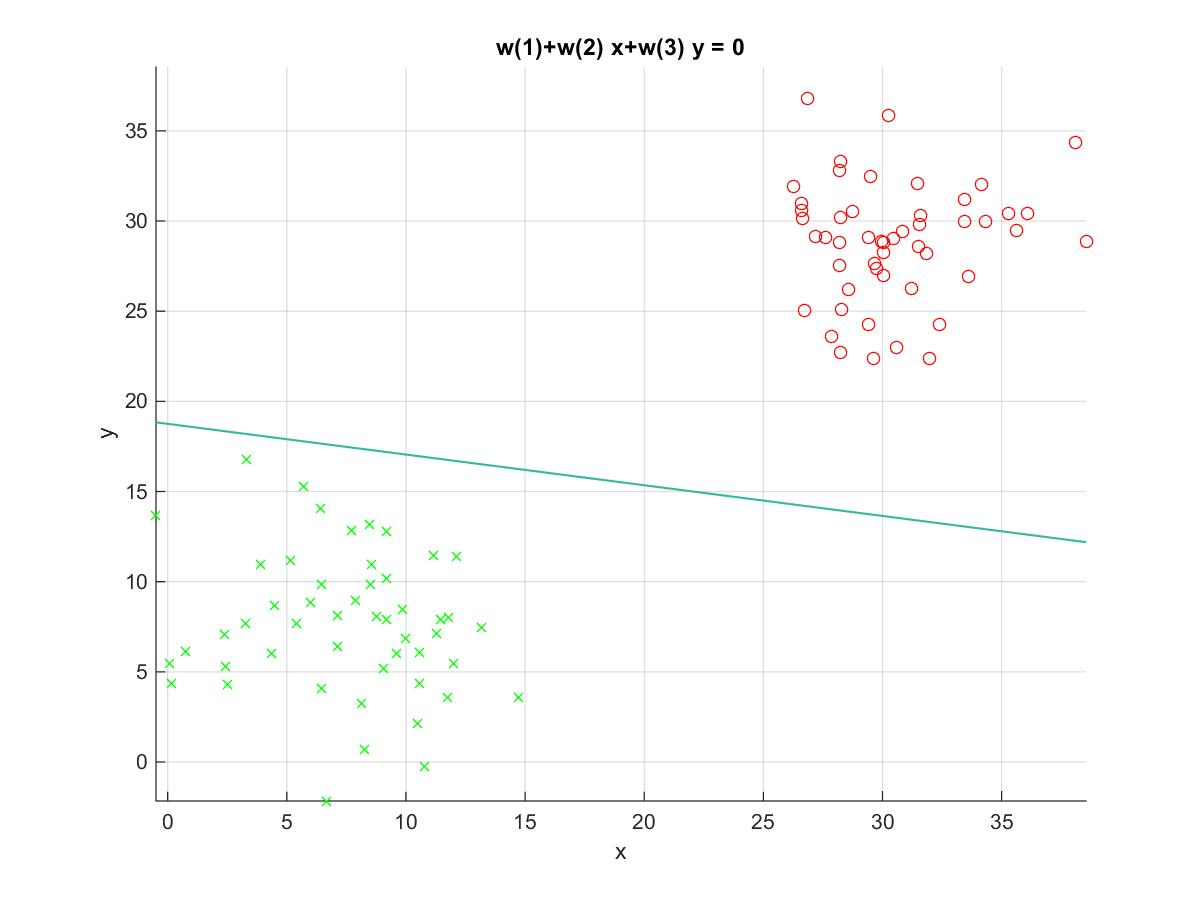
\includegraphics[width=0.7\textwidth]{./images/MyPerceptron_3.jpg}
\caption{Datensatz 1: $\mu_1=10$, $\Sigma_1=3$ , Datensatz 2: $\mu_2=2$, $\Sigma_2=4$}
\end{figure}

\begin{figure}[p]
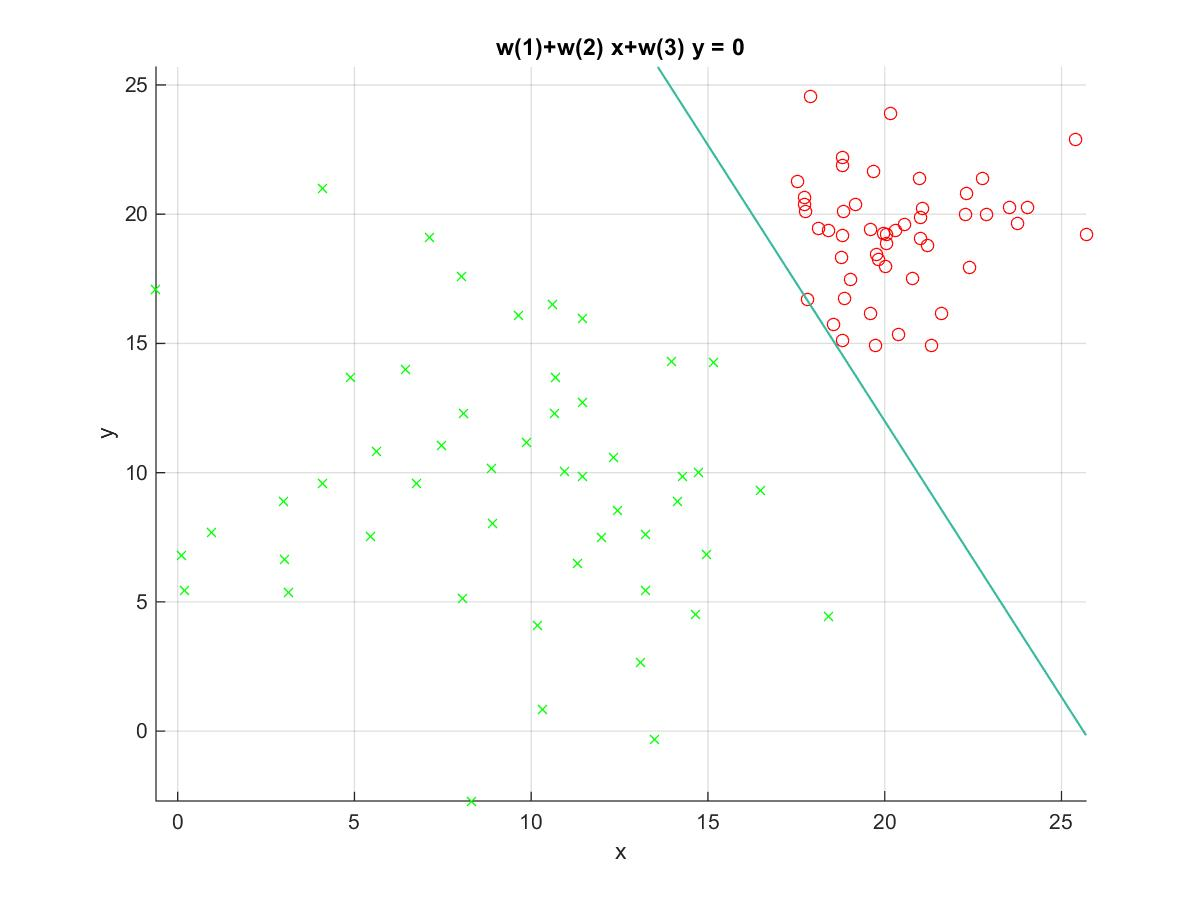
\includegraphics[width=0.7\textwidth]{./images/MyPerceptron_4.jpg}
\caption{Datensatz 1: $\mu_1=10$, $\Sigma_1=2$ , Datensatz 2: $\mu_2=2$, $\Sigma_2=5$}
\end{figure}


\subsection{Wie ist das Verhalten bei nicht linear separierbaren Daten}

Der Algorithmus terminiert nicht da bei jedem Durchlauf Daten gefunden werden, welche in der falschen Klasse landen.

\end{document}          
